\chapter{Filtri di Bloom}

\section{Problema dell'Approximate Set Membership}
Il problema affrontato dai filtri di Bloom (BF) è quello dell'Approximate Set Membership (ASM) (\cite{bloom1970}), che riguarda la verifica dell'appartenenza di un elemento $x \in \mathcal{U}$ a un insieme noto $S \subset \mathcal{U}$, i cui elementi prendono il nome di \textit{chiavi}. L'insieme universo $\mathcal{U}$ non è altro che l'insieme di tutti i possibili elementi di cui si potrebbe valutare l'appartenenza a un sottoinsieme $S$. Ad esempio, se $S$ contenesse numeri interi, $\mathcal{U}$ coinciderebbe con $\mathbb{Z}$. 

L'obiettivo, quindi, è progettare un filtro efficiente sia in termini di memoria occupata che di tempi di risposta, che possa rispondere alla domanda:  
\begin{center}
    \textit{$x$ è una chiave?}
\end{center}
L'efficienza è il requisito centrale di queste strutture: si predilige un filtro efficiente che risolva il problema in modo approssimato, cioè non garantendo la massima accuratezza nel rispondere alla domanda di cui sopra, a un filtro esatto che deve necessariamente memorizzare al suo interno tutte le chiavi.

In particolare, è tollerato che il filtro possa occasionalmente giudicare come chiave un elemento che non lo è (caso di falso positivo), ma non deve mai escludere un elemento che appartiene effettivamente a $S$ (falso negativo). Per questo il tasso di falsi positivi di un filtro ne costituisce una caratteristica cardinale: rappresenta la misura di quanto si rinuncia in accuratezza per, si auspica, guadagnare in efficienza. Il compromesso principale è dunque quello tra tasso di falsi positivi e spazio occupato.

Poiché il tasso di falsi negativi è garantito essere nullo, questo tipo di filtro viene spesso utilizzato per escludere con certezza un elemento da un insieme.

\section{Applicazioni}
Disporre di una struttura dati di piccole dimensioni che può rapidamente escludere un elemento da un insieme rappresenta un vantaggio in numerosi contesti. In genere, ovunque ci sia un database di grandi dimensioni che venga frequentemente interrogato sull'esistenza di un particolare record, un filtro di questo tipo ha un impatto positivo sulle prestazioni, in quanto permette di evitare letture inutili qualora il record cercato non sia presente.

In ambito di sicurezza in rete, si può classificare un URL come sicuro senza dover consultare direttamente l'archivio contenente gli indirizzi malevoli (\cite{patgiri2021deepbf}).
Nei sistemi peer-to-peer o nei database distribuiti, si riduce la quantità di informazioni scambiate in rete verificando rapidamente quali elementi sono già presenti in un nodo remoto prima di sincronizzare i dati (\cite{broder2004network}). Nei sistemi di caching, si evitano letture inutili della cache (\cite{maggs2015algorithmic}).

\section{Definizione e Costruzione di un BF}

Un BF consiste in un vettore $\mathbf{b}$ di $m$ bit e in $k$ funzioni di hash $h_1, \dots, h_k$ indipendenti tra loro e uniformi sul codominio, dato da $\{1, \dots, m\}$. Ossia, ciascuna funzione mappa ogni elemento $x \in \mathcal{U}$ in una delle $m$ posizioni del vettore; a ciascun elemento sono dunque associati $k$ bit.

Inizialmente, quando nessuna chiave è stata aggiunta al filtro, tutti i bit di $\mathbf{b}$ valgono 0. \\
Per aggiungere una chiave, si impostano a 1 i bit a essa associati (chiaramente, se almeno una chiave è già stata registrata nel BF, può darsi che uno o più bit abbiano già valore 1; in questo caso, vengono lasciati a 1). Questo fa in modo che, per qualsiasi elemento, avere tutti i bit associati con valore 1 sia una condizione necessaria per essere chiave.

Per verificare se un elemento sia una chiave o no, si osservano i corrispondenti bit: se almeno uno ha valore 0, l'elemento sicuramente non è una chiave; altrimenti potrebbe esserlo. Infatti, potrebbe capitare che tutti i bit relativi all'elemento oggetto di verifica siano stati impostati a 1 durante l'aggiunta di altre chiavi. In questo caso, il filtro commette un falso positivo. Conoscere il tasso di falsi positivi del filtro significa conoscere la probabilità con cui questo caso si presenta.

\subsubsection{Esempio}
Consideriamo un BF avente un vettore $\mathbf{b}$ di 15 posizioni, inizialmente vuoto.

\begin{center}
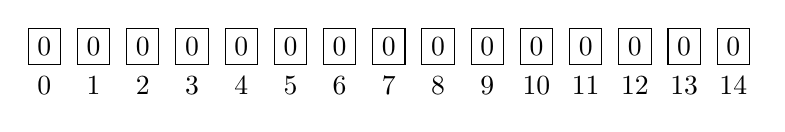
\begin{tikzpicture}
    % Definiamo quali bit devono essere impostati a 1
    \def\bitston{{0, 0, 0, 0, 0, 0, 0, 0, 0, 0, 0, 0, 0, 0, 0}} 

    % Disegna i quadrati rappresentanti i bit
    \foreach \i in {0,...,14} {
        \node[draw, minimum size=0.4cm] at (\i/1.6, 0) {\pgfmathparse{\bitston[\i]}\pgfmathresult}; % Inserisce 0 o 1 nel quadrato
        \node at (\i/1.6, -0.5) {\i}; % Etichetta con il numero della posizione
    }
\end{tikzpicture}
\end{center}

Siano $c_1$, $c_2$ e $c_3$ le chiavi da inserire, ossia gli elementi di $S$. Per ogni chiave, utilizziamo 2 funzioni di hash, denominate $h_1$ e $h_2$, che restituiscono indici nell'insieme $\{0, \dots, 14 \}$. Supponiamo che le funzioni di hash restituiscano i seguenti valori per le chiavi:
\begin{equation}
    \begin{aligned}
        & h_1(c_1) = 3, \quad h_2(c_1) = 8 \\
        & h_1(c_2) = 6, \quad h_2(c_2) = 12 \\
        & h_1(c_3) = 8, \quad h_2(c_3) = 14 \enspace . \\
    \end{aligned}
\end{equation}

I bit che vanno impostati a 1 sono dunque quelli nelle posizioni 3, 6, 8, 12 e 14.

\begin{center}
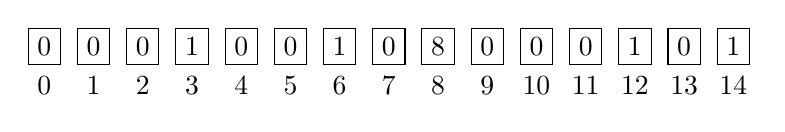
\begin{tikzpicture}
    % Definiamo quali bit devono essere impostati a 1
    \def\bitston{{0, 0, 0, 1, 0, 0, 1, 0, 8, 0, 0, 0, 1, 0, 1}} 

    % Disegna i quadrati rappresentanti i bit
    \foreach \i in {0,...,14} {
        \node[draw, minimum size=0.4cm] at (\i/1.6, 0) {\pgfmathparse{\bitston[\i]}\pgfmathresult}; % Inserisce 0 o 1 nel quadrato
        \node at (\i/1.6, -0.5) {\i}; % Etichetta con il numero della posizione
    }
\end{tikzpicture}
\end{center}

Supponiamo ora di dover classificare una non-chiave, $x_1$, e che si abbia:
\begin{equation}
    h_1(x_1)=3, \quad h_2(x_1)=7 \enspace.
\end{equation}
Dal momento che $b_3 = 1$ ma $b_7 = 0$, possiamo correttamente affermare che $x \notin S$.


\section{Analisi di un BF}
\label{par:analisi-bf}

Conoscendo il numero di funzioni di hash, $k$, la dimensione del vettore, $m$, e il numero di chiavi, $n$, possiamo stimare il tasso di falsi positivi $\epsilon$ di un BF.

Essendo le funzioni di hash uniformi sul codominio, presa una singola funzione, la probabilità che un bit qualsiasi del vettore non sia selezionato da essa, e che quindi rimanga a 0 durante l'aggiunta di una sola chiave è

\begin{equation}
    1 - \frac{1}{m} \enspace.
\end{equation}

Dal momento che le funzioni di hash sono anche indipendenti tra loro, possiamo affermare che la probabilità che tale bit non sia selezionato da nessuna di esse è 

\begin{equation}
    \left( 1 - \frac{1}{m} \right)^k \enspace.
\end{equation}

Sfruttando l'identità

\begin{equation}
    \lim_{m \to \infty} \left( 1 - \frac{1}{m} \right)^m = e^{-1}
\end{equation}

\noindent possiamo affermare che, per $m$ grandi, 

\begin{equation}
    \left( 1 - \frac{1}{m} \right)^k = \left[ \left( 1 - \frac{1}{m} \right)^m \right] ^ {k/m} \approx e^{-k/m} .
\end{equation}

Se inseriamo $n$ chiavi, la probabilità che un singolo bit rimanga a 0 è 

\begin{equation}
    p= \left( 1 - \frac{1}{m} \right)^{kn} \approx e^{-kn/m} .
\end{equation}

La probabilità che un bit qualsiasi venga impostato a 1 durante l'aggiunta delle chiavi è quindi $1-p$. Ne consegue che la probabilità che $k$ bit siano tutti casualmente impostati a 1 durante l'aggiunta delle chiavi sia $(1-p)^k$ (stiamo assumendo che i valori dei singoli bit siano indipendenti tra loro, semplificando).
Questa non è altro che la probabilità di commettere un falso positivo nel valutare una non-chiave. Tale probabilità coincide col tasso di falsi positivi:

\begin{equation}
    \epsilon = (1-p)^k \approx (1-e^{-kn/m})^k .
    \label{expr:fpr-prob}
\end{equation}

Da notare che questo ragionamento probabilistico non è valido per le chiavi: i bit associati a una chiave non sono casualmente impostati a 1; lo sono per costruzione. Tutti i bit relativi a una chiave hanno sempre valore 1.

Da (\ref{expr:fpr-prob}) possiamo evincere che $\epsilon$ aumenta all'aumentare di $n$ e diminuisce all'aumentare di $m$ (facendo variare rispettivamente solo $n$ e $m$).

Possiamo anche giungere al valore ottimo di $k$ avendo $n$ e $m$. Tenuto conto della relazione tra $p$, $k$, $n$ e $m$ si ha:

\begin{equation}
    \ln{\epsilon} = \ln{((1-p)^k)} = k \ln{(1-p)} = -\frac{m}{n} \ln{p} \ln{(1-p)} .
\end{equation}

Essendo il logaritmo una funzione monotona crescente, minimizzando $\ln{\epsilon}$, minimizziamo anche $\epsilon$, cosa evidentemente auspicabile. Avendo fissato $m$ e $n$, l'unica variabile rimanente è $p$ (e quindi implicitamente $k$), ed è facile concludere, per simmetria, che l'espressione di cui sopra è minimizzata per $p = \frac{1}{2}$. Da qui si può ricavare $k$ ottimale:

\begin{equation}
    k = -\frac{m}{n} \ln{p} = -\frac{m}{n} \ln{\frac{1}{2}} = \frac{m}{n} \ln{2} .
\end{equation}

Sostituendo in (\ref{expr:fpr-prob}) e sapendo che per $k$ ottimo si ha $p = \frac{1}{2}$ otteniamo:

\begin{equation}
    \epsilon = (1-p)^k \approx \left( \frac{1}{2} \right)^{\frac{m}{n} \ln{2}} ,
\end{equation}

\noindent che può essere semplificata, assumendo anche $p = e^{-kn/m}$, come

\begin{equation}
    \ln{\epsilon} = -\frac{m}{n} \ln^2 2 .
    \label{expr:bf-params}
\end{equation}

Questa espressione evidenzia come, scegliendo $k$ in maniera ottimale, bastino due dei tre parametri $n$, $m$ e $\epsilon$ per ricavare il terzo. Nella maggior parte dei casi, si conosce il numero di chiavi e si fissa un tasso di falsi positivi ritenuto accettabile, per poi determinare la dimensione ottimale del vettore, ossia lo spazio occupato dal filtro. Manipolando (\ref{expr:bf-params}) si ottiene:

\begin{equation}
    m = \left\lceil - \frac{n\ln{\epsilon}}{\ln^2 2} \right\rceil ,
\end{equation}

\noindent dove utilizziamo la parte intera in quanto si tratta di spazio occupato in bit.

Ad esempio, avendo $n=10^4$ chiavi e fissando $\epsilon=0.05$, il filtro occupa

\begin{equation}
    m = \left\lceil - \frac{10^4 \ln 0.05}{\ln^2 2} \right\rceil = 47926 \text{ bit}
\end{equation}

\noindent e il numero di funzioni di hash che impiega è

\begin{equation}
    k = \left\lceil \frac{m}{n} \ln 2 \right\rceil = \left\lceil \frac{47926}{10^4} \ln 2 \right\rceil = 4 \space .
\end{equation}

Per giungere a questi risultati abbiamo adottato diverse approssimazioni e semplificazioni (ognuna di esse è stata segnalata), che tuttavia, nella pratica, non compromettono in modo significativo l'affidabilità delle stime, mantenendo un'adeguata precisione nell'analisi delle prestazioni.

Per quanto riguarda l'aspetto temporale, i BF vantano una particolare proprietà: il tempo necessario per aggiungere chiavi o per classificare elementi è una costante completamente indipendente dal numero di chiavi già inserite: $O(k)$. Ciò è dovuto al fatto che, in entrambe le circostanze, il tempo impiegato è quello necessario a invocare le $k$ funzioni di hash. Peraltro, in un'implementazione hardware, queste invocazioni possono essere parallelizzate.